%%%%%%%%%%%%%%%%%%%%%%%%%%%%%%%%%%%%%%%%%%%%%%%%
% Vektorräume
%%%%%%%%%%%%%%%%%%%%%%%%%%%%%%%%%%%%%%%%%%%%%%%%
\section{Vektorräume}

\subsection{Rechenregeln und Definition}
	\begin{tabular}{| l | l |}
		\hline v0: & $a + b = b + a$\\
			& $a + (b + c) = (a + b) + c$\\
		\hline v1: & $0 \in \mathbb{R}, 0 = (0, \ldots, 0) \qquad v + 0 = v \qquad \forall v$\\
		\hline v2: & zu $v \in \mathbb{R}^n$ gibt es ein $-v = (-v_1, \ldots, -v_n)$ \qquad mit $v + (-v) = 0$\\
		\hline v3: & $0 \cdot v = 0 \qquad 1 \cdot v = v$\\
		\hline v4: & $\lambda(u + v) = \lambda u + \lambda v$\\
			& $(\lambda + \mu) \cdot u = \lambda u + \mu u$\\
			& $(\lambda\mu)u = \lambda(\mu u)$\\
		\hline
	\end{tabular}\\ \\

	\textbf{Def.:} Eine Menge $V$ mit den Rechenregeln v0-v4 heisst Vektorraum, $v \in V$ heissen Vektoren.

\subsection{lineare Approximation}
	\begin{equation*}
		\left(\begin{array}{c}
			a_0 + a_1x_0 + a_2{x_0}^2 + \ldots + a_n{x_0}^n\\
			a_0 + a_1x_1 + a_2{x_1}^2 + \ldots + a_n{x_1}^n\\
			\vdots \\
			a_0 + a_1x_n + a_2{x_n}^2 + \ldots + a_n{x_n}^n\\
		\end{array}\right) = \left(\begin{array}{c}
			f(x_0)\\
			f(x_1)\\
			\vdots\\
			f(x_n)
		\end{array}\right) \Rightarrow \left(\begin{array}{ccccc}
			1 & x_0 & {x_0}^2 & \ldots & {x_0}^n\\
			1 & x_1 & {x_1}^2 & \ldots & {x_1}^n\\
			\vdots & \vdots & & \vdots \\
			1 & x_n & {x_n}^2 & \ldots & {x_n}^n\\
		\end{array}\right) \cdot \left(\begin{array}{c}
			a_0\\
			a_1\\
			\vdots \\
			a_n
		\end{array}\right) = \left(\begin{array}{c}
			f(x_0)\\
			f(x_1)\\
			\vdots \\
			f(x_n)
		\end{array}\right)
	\end{equation*}

\subsection{Spur}
	Die Spur ist die Summe der Diagonalelemente einer Matrix $Spur(A) = \Sigma a_{ii}$\\
	$Spur(ABC) = Spur(CAB) = Spur(BCA) \rightarrow$ zyklisch vertauschbar


\subsection{Basis}
	\textbf{Def.:} Sei also $V$ ein Vektorraum. Eine Menge $B = \lbrace b_1, b_2, \ldots \rbrace$ linear unabhängiger Vektoren
	ist eine Basis, wenn jeder Vektor von $V$ als Linearkombination von Vektoren aus $B$ dargestellt werden kann. Ein 
	Vektorraum heisst endlichdimensional, wenn er eine endliche Basis hat. 

\subsection{Basistransformation}
	\begin{minipage}{7cm}
		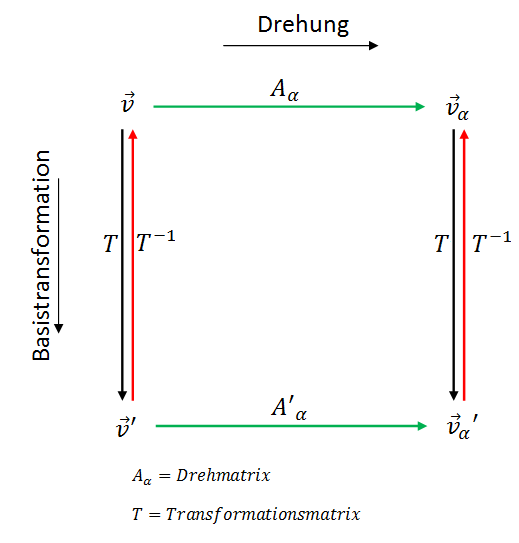
\includegraphics[width=7cm]{pics/2_Basistransformation.png}
	\end{minipage}
	\begin{minipage}{7cm}
		\begin{tabular}{ll}
			& $A =$ Matrix in alter Basis\\
			$A' = TAT^{-1}$ & $A' =$ Matrix in neuer Basis\\
			& $T =$ Transformationsmatrix\\
			$\xi' = T\xi$& $\xi =$ Vektor in der alten Basis\\
			& $\xi' =$ Vektor in der neuen Basis
		\end{tabular}
	\end{minipage}

	\subsubsection{Bestimmen der Transformationsmatrix $T$}
		$B = \underbrace{\lbrace b_j \rbrace}_{alte Basis} \qquad B' = \underbrace{\lbrace b_j' \rbrace}_{neue Basis}$\\ \\

		\textbf{Variante 1 (mit $\beta$):}\\
		Mit Gleichungssystem herausfinden, wie viele von der neuen Basis gebraucht wird um die alte darzustellen.\\
		$b_j = \beta_{j1}b_1' + \beta_{j2}b_2' + \ldots + \beta_{jn}b_n' \rightarrow$ daraus folgt $\beta$\\
		\begin{equation*}
			\mathbf{T = \beta^t}
		\end{equation*}

		\textbf{Variante 2:}\\
		Oftmals ist $b_j'$ mit den Koordinaten von der alten Basis angegeben\\
		$b_j' = \beta_{j1}b_1 + \beta_{j2}b_2 + \ldots + \beta_{jn}b_n$\\
		$\Rightarrow$ Koordinaten in der alten Basis von $b_j'$ in die Spalten der Matrix einfüllen, welches gleich $\mathbf{T^{-1}}$ ist.\\
		\begin{equation*}
			\mathbf{T = (T^{-1})^{-1}}
		\end{equation*}

	\subsubsection{Eigenschaften einer Basistransformation}
		Ein Basiswechsel ändert die Spur und die Determinante nicht!\\
		\begin{equation*}
			Spur(TAT^{-1}) = Spur(T^{-1}TA) = Spur(A)
		\end{equation*}
		\begin{equation*}
			det(TAT^{-1}) = det(T^{-1}) \cdot det(A) \cdot det(T) = det(A)
		\end{equation*}

\subsection{Lineare Abbildungen}
	\subsubsection{Orientierung}
		\begin{tabular}{lp{13cm}}
			$GL_n(\mathbb{R}) = \lbrace A | det(A) \neq 0\rbrace$ & "general linear group'' enthält alle lineare Abbildungen\\
			& $det(A)\left\lbrace\begin{array}{cc}
				>0 & \text{Rechtssystem}\\
				<0 & \text{Linkssystem}
				\end{array}\right.$ \\ \\

			$SL_n(\mathbb{R}) = \lbrace A | det(A) = 1 \rbrace$ &  ''special linear group'' enthält alle volumen- und orientierungstreue Matrizen\\
			& $det(A) =$ Volumenänderungsfaktor \\ \\

			$O(n) = \lbrace A | A^tA = E \rbrace$ & enthält alle orthogonalen Matrizen, die Längen und Winkel bleiben erhalten.\\
			& Die Detereminante ist dabei $det(A) = \pm1$ (Zeilen-/Spaltenvektoren sind orthogonal) ($OO^t = E$)
		\end{tabular}\\ \\

		\begin{tabular}{ll}
			$SO(n) = \lbrace A \in GL_n(\mathbb{R}) | det(A) = 1, A^tA = E \rbrace$ & Drehmatrizen, Volumen, Längen und Winkel bleiben 					erhalten.
		\end{tabular}

	\subsubsection{Drehwinkel}
		\begin{tabular}{p{5cm}l}
			in $SO(2)$ & \begin{equation*}
				\cos\alpha = \frac{Spur(D_\alpha)}{2}
			\end{equation*} \\ \\
			
			in $SO(3)$ ohne Spiegelung & \begin{equation*}
				\cos\alpha = \frac{Spur(D_\alpha) - 1}{2}
			\end{equation*}\\ \\

			 in $SO(3)$ mit Spiegelung & \begin{equation*}
				\cos\alpha = \frac{Spur(D_\alpha) + 1}{2}
			\end{equation*}
		\end{tabular}
		
	\subsubsection{einige Lineare Abbildungen}
		\begin{tabular}{llll}
			$A=	\left(\begin{array}{ll}0 &1 \\1 &0\end{array}\right)$ 
        			&$\Rightarrow$ Spiegelung an Geraden $x_2=x_1$
			&$A=	\left(\begin{array}{ll}0 &-1 \\1 &0\end{array}\right)$ 
            		&$\Rightarrow$ Drehung um $\vec{O}$ mit $+90^{\circ}$\\
			$A=	\left(\begin{array}{ll}1 &1 \\0 &1\end{array}\right)$ 
            		&$\Rightarrow$ Scherung $\|$ zur $x_1$-Achse um $45^{\circ}$
			&$A=	\left(\begin{array}{ll}\cos{\alpha} &-\sin{\alpha} \\\sin{\alpha} &\cos{\alpha}\end{array}\right)$ 
            		&$\Rightarrow$ Drehung um $\vec{O}$ mit $\alpha$\\			
			$A=	\left(\begin{array}{llc}1 &0 &0 \\0 &1 &0 \\0 &0 &-1\end{array}\right)$ 
            		&$\Rightarrow$ Spiegelung  $x_1x_2$ -Ebene
			&$A=	\left(\begin{array}{lll}-1 &0 &0 \\0 &-1 &0 \\0 &0 &-1\end{array}\right)$ 
            		&$\Rightarrow$ Punktspiegelung an $\vec{O}$\\	
			$A=	\left(\begin{array}{lll}2 &0 &0 \\0 &2 &0 \\0 &0 &2\end{array}\right) $
			&$\Rightarrow\begin{array}{l}\mbox{Streckung von } \vec{O} \mbox{ aus} \\ \mbox{mit Faktor 2} \end{array}$
			&$A=	\left(\begin{array}{lll}\cos{\alpha} &-\sin{\alpha} &0 \\ \sin{\alpha}
			&\cos{\alpha} &0 \\0 &0 &1\end{array}\right)$ 
			&$\Rightarrow \begin{array}{l}\mbox{Drehung des Raumes}\\ \mbox{um die } x_3
			\mbox{-Achse mit } \alpha \end{array}$										
		\end{tabular}

	\subsubsection{Algebraische Eigenschaften von linearen Abbildungen}
		\begin{minipage}{10cm}
			\begin{tabular}{ll}
				$A \cdot B \neq B \cdot A$ & (Anti-Kommunitativgesetz)\\
				$(A \cdot B)C = A(B \cdot C) = A \cdot B \cdot C$ & (Assoziativgesetz)
			\end{tabular}\\ \\
			\textbf{Verkettung von lin. Abbildungen}\\
			\textbf{$\rightarrow$ Zeile mal Spalte}\\
				$$C=B\circ A=B(A(\vec{x}))$$
		\end{minipage}
		\begin{minipage}{7cm}
			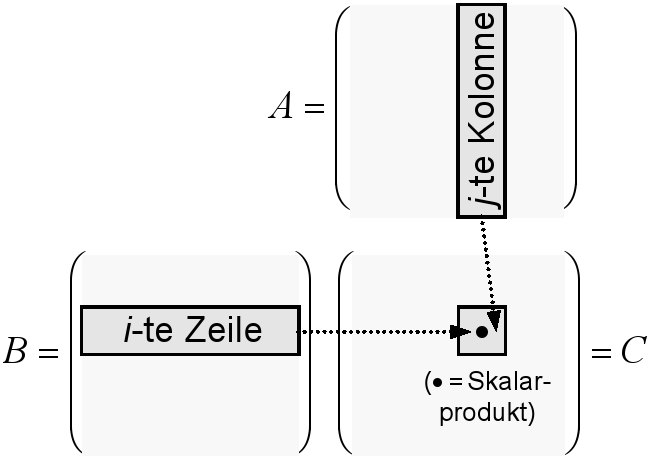
\includegraphics[width=5cm]{pics/3_Matrizenmulti}
		\end{minipage}

\subsection{Allgemeines Skalarprodukt}
	\begin{tabular}{ll}
		$\xi \bullet  \gamma = \xi^tG\gamma$ & $\xi, \gamma$ sind Vektoren\\
		$\xi' \bullet \gamma' = {\xi'}^tG'\gamma' = \xi^tT^tG'T\gamma$ & G = Symmetrische Matrix\\
		$G = T^tG'T$ & G in Standartbasis = Einheitsmatrix (E)\\
		$G' = {T^{-1}}^tGT^{-1}$ &
	\end{tabular}





















